%%%%%%%%%%%%%%%%%%%%%%% file template.tex %%%%%%%%%%%%%%%%%%%%%%%%%
%
% This is a general template file for the LaTeX package SVJour3
% for Springer journals.          Springer Heidelberg 2010/09/16
%
% Copy it to a new file with a new name and use it as the basis
% for your article. Delete % signs as needed.
%
% This template includes a few options for different layouts and
% content for various journals. Please consult a previous issue of
% your journal as needed.
%
%%%%%%%%%%%%%%%%%%%%%%%%%%%%%%%%%%%%%%%%%%%%%%%%%%%%%%%%%%%%%%%%%%%
%
% First comes an example EPS file -- just ignore it and
% proceed on the \documentclass line
% your LaTeX will extract the file if required
\begin{filecontents*}{example.eps}
%!PS-Adobe-3.0 EPSF-3.0
%%BoundingBox: 19 19 221 221
%%CreationDate: Mon Sep 29 1997
%%Creator: programmed by hand (JK)
%%EndComments
gsave
newpath
  20 20 moveto
  20 220 lineto
  220 220 lineto
  220 20 lineto
closepath
2 setlinewidth
gsave
  .4 setgray fill
grestore
stroke
grestore
\end{filecontents*}



%
\RequirePackage{fix-cm}
%
%\documentclass{svjour3}                     % onecolumn (standard format)
%\documentclass[smallcondensed]{svjour3}     % onecolumn (ditto)
\documentclass[smallextended]{svjour3}       % onecolumn (second format)
%\documentclass[twocolumn]{svjour3}          % twocolumn
%
\smartqed  % flush right qed marks, e.g. at end of proof
%\begin{document}
\usepackage{graphicx}

\usepackage{caption}
\usepackage{subfig}

\usepackage{cite} 
\usepackage[main=english, spanish]{babel}
%\usepackage[utf8]{inputenc}

\usepackage{amssymb, amsmath, amsbsy} % simbolitos
\usepackage{upgreek} % para poner letras griegas sin cursiva
\usepackage{cancel} % para tachar
\usepackage{mathdots} % para el comando \iddots
\usepackage{mathrsfs} % para formato de letra
\usepackage{stackrel} % para el comando \stackbin
\renewcommand{\tablename}{Table} 
\renewcommand{\figurename}{Figure} 
%

\usepackage{url}
\usepackage{mathptmx}      % use Times fonts if available on your TeX system
%
% insert here the call for the packages your document requires
%\usepackage{latexsym}
% etc.
%
% please place your own definitions here and don't use \def but
% \newcommand{}{}
%
% Insert the name of "your journal" with
% \journalname{myjournal}
%
\begin{document}

\providecommand\foo{}
\renewcommand\foo{...}


\title{Context-Aware Recommender System Using Post-Filtering And Fuzzy Logic
}
\subtitle{}

%\titlerunning{Short form of title}        % if too long for running head

\author{Xochilt Ramirez-Garcia \and Mario Garcia-Valdez %etc.
}

%\authorrunning{Short form of author list} % if too long for running head

\institute{Xochilt Ramirez-Garcia \at
              \email{xochilt.ramirez@gmail.com}           %  \\
%             \emph{Present address:} of F. Author  %  if needed
           \and
           Mario Garcia-Valdez\at
             mario@tectijuana.edu.mx
}

\date{Received: date / Accepted: date}
% The correct dates will be entered by the editor

\maketitle

\begin{abstract} 
%Al último revisamos el abstract
Contextual recommendations are implemented in recommender systems to improve
user satisfaction. A recommender system makes accurate and suitable
recommendations for a particular situation reaching personalized
recommendations.
%%Mario: Creo que es mejor empezar aqui:
The context provides information relevant to the recommender
system and is used as a filter for selection of relevant items for the user.

This paper presents a context-aware recommender system, which uses techniques
based on collaborative filtering and content-based as well as fuzzy rules to
recommend items in context. The dataset used to test the system is Trip Advisor.
The accuracy in the recommendations was evaluated with the Mean Absolute Error.

\keywords {Algoritms \and Content-based\and Context \and  Collaborative filtering\and  
Fuzzy logic \and  Recommender systems} 
% \PACS{PACS code1 \and PACS code2 \and
% \subclass{MSC code1 \and MSC code2 \and more} \end{abstract}
\end{abstract}

\section{Introduction} \label{intro} 

Nowadays, Internet provides users convenient tools to improve tasks in daily
life in order to know the needs of millions of users, this has disadvantages
that leads to information overload . % al revés
For example, an online store can offer
thousands of items in different categories for the user, as result, the user
could find in a complex situation, where the items that the user want to buy are
contained in a list of thousands of items in the online store. Then, recommender
systems are designed for suggest items that are adapted to needs and preferences
of users \cite{ricci2011introduction}. 

There are two common  techniques for
recommendations: 1) collaborative filtering and, 2) content-based. These
algorithms can be combined in a hybrid system \cite{burke2007hybrid}.   The
highlight of traditional recommender systems is that considers only two types of
entities (users and items) with no taking in account the context. Subsequently,
in a way to improve these recommender systems, the efforts are based in the
integration of the context in the recommendation process, someway. For example,
the use of applications such as recommendation of restaurants
\cite{ramirez2014post}, sightseeing \cite{baltrunas2011},
\cite{baltrunas2011context}, personalized content on a web page
\cite{marina2010ontology}, a movie \cite{kim2010recommender}, or a song list
\cite{baltrunas2011incarmusic}, it can be insufficient to consider only
information about users and items, it is important contextual information in the
referral process in order to recommend items in specific circumstances or
situations \cite{zimmermann2000personalization}.  When context is added in an
application, context-aware recommender systems meet its  function to get
suitable items for users, specially when the context information has a high
relevance for the domain such as in \cite{baltrunas2011context}.  For achieve
this purpose, researchers propose new techniques such as in
\cite{said2011inferring},\cite{zheng2014splitting} and
\cite{baltrunas2009context2} , where a splitting of rating matrix is used to
sepate the context and it adjust it in recommendation process.  

In recent works
such as \cite{zhengcorrelation} and \cite{baltrunas2011matrix} , the matrix
factorization technique have been improved for adding context, getting better
results than standard matrix factorization technique \cite{koren2009matrix}.
Subsequently, have been developed location-aware recommender system such as in
\cite{levandoski2012lars} and \cite{kaminskas2011location}, because of the
importance of the location factor when the items are recommended taking in
account the user geographical position and the distance of items such as
restaurants or some places of interest. The time factor has a high impact in
recommender systems due to the changes that happen in a context throuhg the
time, such that nowadays time-aware recommender systems \cite{hamed2012t} are
integrated in new mobile applications such as InCarMusic
\cite{baltrunas2011incarmusic},  ReRex \cite{baltrunas2011mobile},  UbiquiTOUS
\cite{bellavista2012survey} and Appazaar \cite{bohmer2010contextualizing} in
order to meet the needs of users. \\

The content of this paper is presented as
follows: section 2 describes the techniques for Recommender Systems, section 3
explains the elements of the method proposed for Context- Aware Recommender
System, section 4 describe the settings of development environment, the datasets
used to test the Context-Aware Recommender System, section 5 explains the
results of experiments to evaluate the system, the main features of the data and
finally, the section 6, explains the conclusions and proposals for future work.
%\cite{hussein2013context}, \cite{kahng2011ranking}.

% A la sección le hace falta corregir el inglés, pero la veo más como el
% estado del arte, en la Intro debes de explicar:
% 1. El problema- creo que eso lo haces bien.
% 2. De manera resumida la justificación de la propuesta. 
% 3. Como está organizado el contenido. 

% Creo que la segunda sección se debería llamar estado del arte.  Y llevarte 
% el segundo párrafo.


\section{ Recommendation techniques } \label{sec:2} 

In recent years, Recommender Systems help to solve the problem of overload
information experienced by consumers on the Internet. Recommender Systems
working with Collaborative Filtering provided recommendations based on the
profile and preferences of users. These Recommender Systems have been tested to
be one of the most used techniques to help users find relevant items for them
\cite{dey2001understanding}, \cite{burke2007hybrid}.

  \subsection{Context-aware recommender systems} \label{sec:2.1}  

  Context-Aware Recommender Systems (CARS) have been developed to solve the
  limitations of traditional Recommender Systems that do not consider the
  context when an item is recommended, for example, to recommend movies
  specifically for Cristmas week \cite{abowd1999towards}. In literature, the
  definition of A. Dey \cite{fischer2012context} about context is widely
  adopted: \textit {"Context is any information that can be used to characterize
  the situation of an entity. An entityis a person, place, or object that is
  considered relevant to the interactionbetween a user and an application,
  including the user and applications themselves."} \\ A context-aware
  recommender system considers contexts, e.g. time, place, companion, etc.,
  using paradigms of recommendation \cite{adomavicius2011context}such as: 1)
  Pre-filtering, where the contexts are used for selecting the data before
  applying the standard CF, 2) Post-filtering, where contexts are incorporated
  for refine the result of CF, and 3) Context modeling, where the context is
  directly integrated to the predictions of the users in the items
  \cite{shani2008mining}. A traditional Recommender System utilizes to represent
  the rating the 2-dimensional function: ${R: (Users \times Items \rightarrow
  Rating)}$, while CARS, add context for  each rating and is represented as a
  multi-dimensional function: \\ ${ R:(Users \times Item \times Context
  \rightarrow Rating)}$.

  \subsection{Collaborative filtering algorithm} \label{sec:2.2}

  This technique obtains specific recommendations for the user, based in ratings
  or usage patterns (e.g. shopping), without exogenous information on any of the
  items or users involved.  As was mentioned in introdution, collaborative filtering uses two entities:
  items and users, but previous to get recommendations for users collaborative filtering gets
  similarity among users. In order to calculate this similarity two approaches
  are proposed: 1) the nearest neighbors and, 2) latent factor model. The
  nearest neighbors approach is based in the relation between items, or users.
  The latent factor model, such as a matrix factorization comprises an
  alternative approach by transforming both elements and the users with the same
  latent factor space. The latent space tries to explain the ratings through
  user and item characterizations, about the inferred factors automatically of
  the user feedback \cite{ricci2011introduction}.

  \subsection{Content-based algorithm} \label{sec:2.3}

  The system learns to recommend items that were relevant for the user in the
  past. The similarity of items is based on the features associated with the items
  compared. For example, if a user liked a comedy film, then the system can learn
  to recommend other comedy films for the same user. This technique analyzes a set
  of documents and descriptions previously rated by the user and makes a user
  profile based on the characteristics of the objects rated by that user. The
  recommendation process basically consists of comparing the attributes of the
  user profile and the attributes of an object, if these attributes are in the
  user profile; this is an advantage to process information. For example, it could
  be used to filter search results to determine if a user is interested or not in
  a specific Web page, if user do not like, it is possible to prevent data from
  that page are displayed\cite{ricci2011introduction}.


  \subsection{Recommendation by popularity} \label{sec:2.4}

  To make recommendations by popularity means consider the popularity of an item
  in the users community \cite{shani2008mining},\cite{celma2008new}, i.e., how
  many people have evaluated a single item. Prediction by popularity works on
  the principle that an item is popular because has been rated by many people,
  it means that can be more informative and relevant within the space of items.


% Que otros algoritmos hibridos existen que se enfoquen al contexto?
% Si lo que se presenta es el sistema de restaurantes, falta hablar de los otros
% Reja, etc.

% Después hablar del problema que vamos a atacar

\section{Proposed method}\label{sec:3}


The proposed method consists of three algorithms to recommend: Fuzzy Inference
System (FIS), collaborative filtering and content-based.   Each one uses rating
matrix to get recommendations. The contetx-aware recommender system uses the
post-filtering paradigm \cite{adomavicius2011context} for adjust
recommendations into the context. The recommendation by popularity is through
the FIS, the FIS contains the variables that are probably involved in a process
to make a suggestion in a human interaction, this process is the same that the
recommender system does. The output represents how matter each item into the
users community, i.e., if it was a popular item for users. The FIS uses fuzzy
rules to infer the inputs  and output (numeric value) that represents the weight
of the recommendation. The FIS has Gaussians membership functions and are
depicted in Fig.\ref{fig:mffis}.


\begin{figure}[ht!]
   \centering
   %%----primera subfigura----
   \subfloat[]{
        \label{fig:1a}
        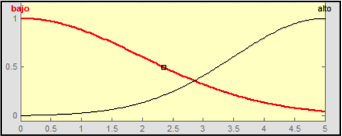
\includegraphics[width=0.42\textwidth]{img/ratingaverage.png}}
   \hspace{0.1\linewidth}
   %%----segunda subfigura----
   \subfloat[]{
        \label{fig:1b} 
        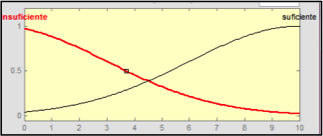
\includegraphics[width=0.42\textwidth]{img/userparticipation.png}}\\[20pt]
   %%----tercera subfigura----
    \subfloat[]{
        \label{fig:1c} 
        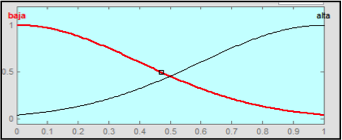
\includegraphics[width=0.42\textwidth]{img/recommendation.png}}
   \caption{Gaussian Membership functions in the input are: a) RatingAverage, 
   b) UserParticipation, and an output: c) Recommendation.}
   \label{fig:mffis} 
\end{figure}

The fuzzy rules in the FIS (Fig.\ref{fig:fis}) are:
\begin{enumerate} 
\item \texttt{If RatingAverage is low and UserParticipation is  insufficient then recommendation is low.}
\item \texttt{If RatingAverage is low and UserParticipation is  sufficient   then recommendation is high.} 
\item \texttt{If RatingAverage is high and UserParticipation is insufficient then recommendation is low.}
\item \texttt{If RatingAverage is high and UserParticipation is sufficient   then recommendation is high.}
\end{enumerate} 

% Se debe justificar el uso del FIS, que ventajas tiene? Que otras opciones hay?
% Se tiene que optimizar? Se puede optimizar? Deberíamos optimizarlo.

% For two-column wide figures use
\begin{figure*}
\captionsetup{justification=centering,margin=2cm}
\centering

\setlength\fboxsep{0pt}
\setlength\fboxrule{0.7pt}
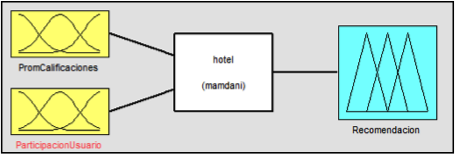
\includegraphics[width=0.75\textwidth]{img/fis.png}
% Use the relevant command to insert your figure file.
% For example, with the graphicx package use
% 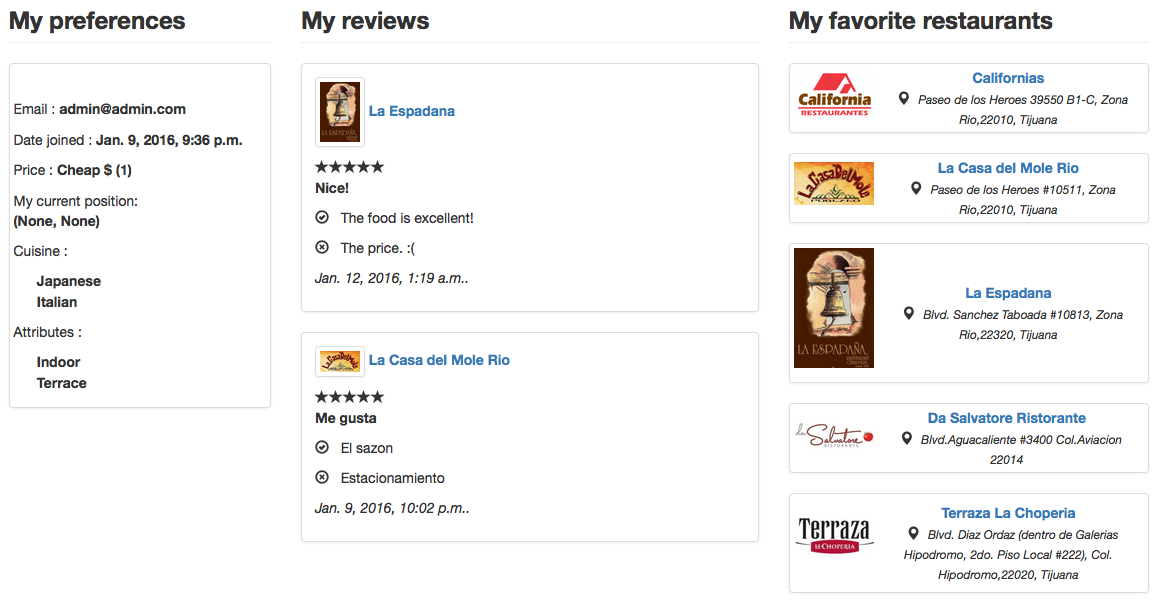
\includegraphics[width=0.75\textwidth]{img/user-profile.png}
% figure caption is below the figure
\caption{Fuzzy Inference System.}
\label{fig:fis}       % Give a unique label
\end{figure*}

Content-based algorithm uses cosine similarity to compare the binary vectors % Debes explicar por que esa medida de similaridad.
representing the profile of each item, thereby obtaining a numerical value that
determines similarity, based on a threshold. In other words, it makes a
comparison of profiles of each item to determine the \textit{most similar} to
items the user has rated with highest score, context-aware recommender system
proposed has a scale from 1.0 to 5.0. The formula of cosine similarity used is
depicted in equation (1).

\begin{equation}
\displaystyle % S(I_{x},I_{y})= 
 Cos (\vec{I_{x}}, \vec{I_{y}}) ={\vec{I_{x}} \cdot  \vec{I_{y}} \over \parallel \vec{I_{x}} \parallel_{2} \cdot \parallel \vec{I_{y}} \parallel_{2}} = {\sum_{i=1}^{n} I_{i,x} I_{i,y} \over \sqrt{\sum_{i=1}^{n} I_{i,x}^{2}} \sqrt{\sum_{i=1}^{n} I_{i,y}^{2}}} 
\end{equation}

Where \textit{CosSim(x,y)} represents the cosine of the angle between the two vectors
(profiles) of the items being compared. Collaborative filtering algorithm
obtains a user neighborhood (KNN-nearest neighbors) and uses the Pearson
correlation for the similarity between neighboring users and the current user,
the \textit{more similar} users will be providing information for the user prediction.
The formula of Pearson correlation \cite{ricci2011introduction} is depicted in equation 2.

\begin{equation}
\displaystyle
P(U_{x}, U_{y}) = {\sum_{i=1}^{n}(U_{xi} - \overline{U})^2 (U_{yi}- \overline{U})^2 \over \sqrt{\sum_{i=1}^{n}(U_{xi}- \overline{U})^2 \sum_{i=1}^{n}(U_{yi}- \overline{U})^2}}
\end{equation}
\\

Where ${P(U_{x}, U_{y})}$ is the correlation coefficient from -1.0 to 1.0, users with the  % De nuevo justificar la correlación
highest positive correlation are considered \textit{more similar}. Then, the process
when collaborative filtering makes predictions \cite{shani2011evaluating} of an item $i$ 
for the user $u$, uses equation 3.

\begin{equation}
P(u,i) = {\sum_{i=1}^{n}(S_{j,u} * C_{j,i}) \over {\sum_{i=1}^{n}(S_{j,u})} }
\end{equation}
\\
Where \textit{P(u,i)} is the prediction for the item \textit{i} for the user
${u, S_{j,u} }$ represents the similarity of the user ${j \in J}$, and
${C_{j,i}}$ is the rating of the user \textit{j} for the item \textit{i}. A
graphic example of a rating matrix used to predict the rating is depicted in
Table \ref{tab:1}.


% For tables use
\begin{table}
\centering
% table caption is above the table
\caption{A rating matrix example.}
\label{tab:1}       % Give a unique label
% For LaTeX tables use
\begin{tabular}{lllll}
\hline\noalign{\smallskip}
Users & Item1 & Item2 & Item3 & Item4  \\
\noalign{\smallskip}\hline\noalign{\smallskip}
User1 & 5 & 4 & 5 & 3  \\
User2 & 4 & 2 & 4 & 5  \\
User3 & 5 & 3 & 5 & Null \\
%number & number & number \\
\noalign{\smallskip}\hline
\end{tabular}
\end{table}


In this example, context-aware recommender system  makes a prediction for
\textit{user3}  on \textit{item4}, using the Pearson correlation coefficient to
determine if the \textit{user1} is more similar to the \textit{user3} than the
\textit{user2}, therefore, uses the profile \textit{user1} (nearest neighbor) to
make a prediction of \textit{3.0} in the \textit{item4} for \textit{user3}. \\In
the next step the outputs of every recommender algorithm is represented by a
list of recommended items. Subsequently apply the context filter and context-
aware recommender system gets the final contextual recommendations. To apply the
context, context-aware recommender system  identifies contextual data of the
user profile (see Table \ref{tab:2}), and compares recommended items to filter
those items that are adjusted to the user context. The context filtering is the
last step before to get the recommended items. The schema of architecture for
context-aware recommender system is depicted in Fig.\ref{fig:architecture}.


\begin{table}[htb]
\centering
\caption{Example of contextual ratings in the user profile.}
\label{tab:2}
\begin{tabular}{lll}
\hline
\multicolumn{3}{c}{User profile} \\ \hline
Item1 & Rating1 & Context1 \\ 
Item2 & Rating2 & Context2 \\ 
Item3 & Rating3 & Context3 \\ \hline
\end{tabular}
\end{table}





% For two-column wide figures use
\begin{figure*}
\captionsetup{justification=centering,margin=2cm}
\centering

%\setlength\fboxsep{0pt}
%\setlength\fboxrule{0.7pt}
\fbox{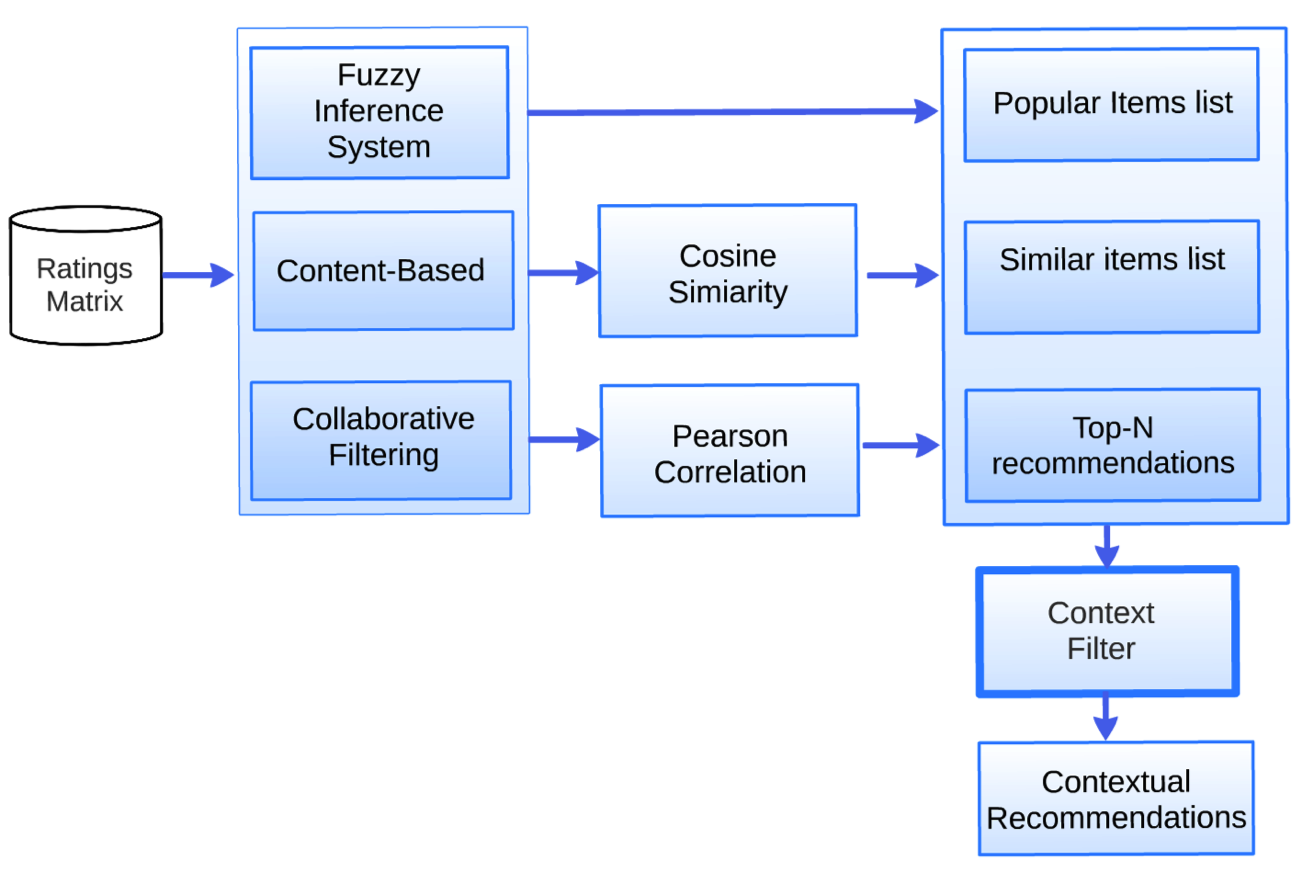
\includegraphics[width=0.70\textwidth]{img/archit.png}}
% Use the relevant command to insert your figure file.
% For example, with the graphicx package use
% 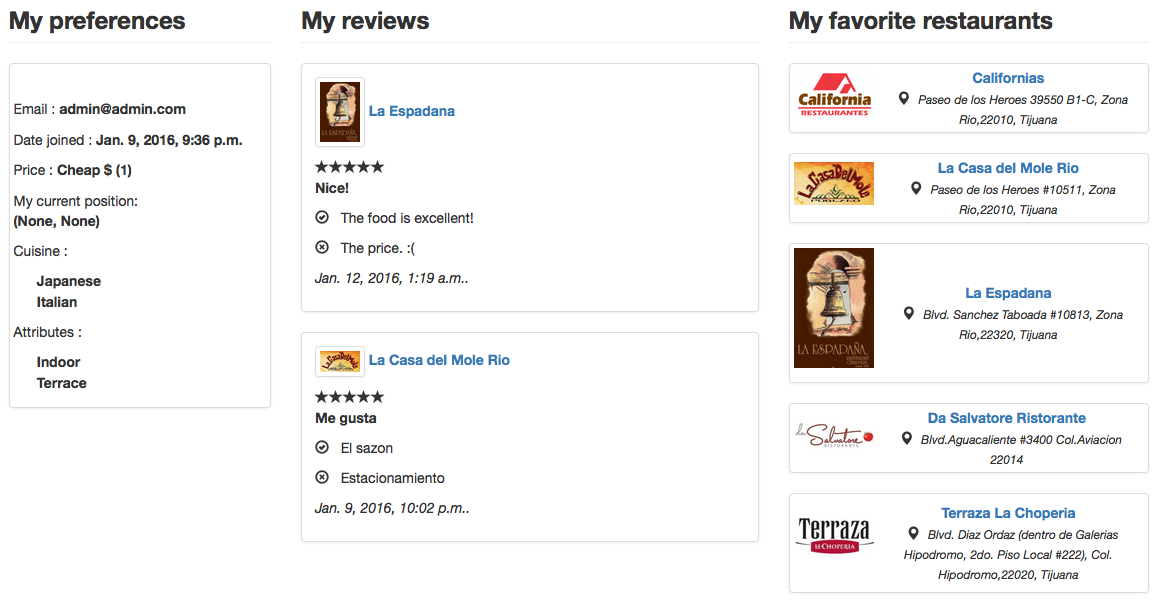
\includegraphics[width=0.75\textwidth]{img/user-profile.png}
% figure caption is below the figure
\caption{Recommender system architecture}
\label{fig:architecture}       % Give a unique label
\end{figure*}



\section{Settings} \label{sec:4}

\subsection{Datasets}\label{sec:4.1}

The dataset used to evaluate the algorithm was TripAdvisor in two versions
downloaded from \cite{linkzeng}, this datasets was used in other papers such as
\cite{zheng2014context}, \cite{zheng2012differential} to evaluate the
performance of context-aware recommender systems. The first dataset contains
4669 contextual ratings 1202 users and 1890 hotels; the second dataset contains
14175 contextual ratings hotels 2731 users and 2269. Data were collected from
reviews online in tripadvisor.com. There is only one context: type of trip
(family, friends, bussines, romantic and relax).


\subsection{Metrics} \label{sec:4.2}

Recommender Systems are widely used in different domains, therefore, the goals
vary for each application, and the evaluation metrics used depend on the general
goals of the system. For some applications the prediction accuracy is essential
and the evaluation of the system is focused on the accuracy of the
recommendations. There are several indicators to measure accuracy: Root Mean
Squared Error (RMSE), Mean Absolute Error (MAE) and, Precision and Recall are
some examples \cite{ricci2011introduction},\cite{campochiaro2009metrics}. On the
other hand, whether the system tries to measure qualitative aspects such as
customer satisfaction, recommendations quality or system utility for a user
group or community, other metrics are considered such as is mentioned in
\cite{campochiaro2009metrics}. \\ The accuracy of prediction is the
controversial property in the literature of recommender systems. The core of the
most of recommender systems is a prediction engine. This engine can predict the
user reviews on the elements (for example of this many researchers have proposed
finding algorithms to provide better predictions in this aspect. The prediction
accuracy is typically independent of the user interface, which can be measured
in an off-line experiment. The precision measuring in a user survey means
accuracy measuring given a recommendation. This is a different concept of
behavior prediction of users without recommendations, and is more accurate
to the accuracy in the real system \cite{ricci2011introduction}.


\section{Results} \label{sec:5}

Two experiments were performed using the dataset described in section 4.1. Table
\ref{tab:3} describes the data sets used and the scarcity percentage of the
specified data. Scarcity of 99 percent mean that there are problems to recommend
items.  \\ By other side, in Table \ref{tab:4} the comparison shows that the
algorithm has a acceptable performance, i.e., the  error falls into the range
of results obtained with others algorithms. Then, contextual recommendations
were evaluated with the Root Mean Square Error in  order to compare the results
with context relaxation algorithm \cite{zheng2012differential} that is evaluated
with the same dataset.

\begin{table}
\centering
% table caption is above the table
\caption{Datasets description.}
\label{tab:3}       % Give a unique label
% For LaTeX tables use
\begin{tabular}{lllll}
\hline\noalign{\smallskip}
Dataset & Users & Items & Ratings & Scarcity (percent) \\
\noalign{\smallskip}\hline\noalign{\smallskip}
TripAdvisor v1 & 1202 & 1890 & 4669 & 99.79 \\
TripAdvisor v2 & 2731 & 2269 & 14175 & 99.77 \\
\noalign{\smallskip}\hline
\end{tabular}
\end{table}




\begin{table}
\centering
% table caption is above the table
\caption{Comparison of RMSE.}
\label{tab:4}       % Give a unique label
% For LaTeX tables use
\begin{tabular}{lll}
\hline\noalign{\smallskip}
Dataset & Algorithm & RMSE \\
\noalign{\smallskip}\hline\noalign{\smallskip}
TripAdvisor v2 & FC + Post-filtering  & 0.504  \\
               & FC          & 0.994  \\
               & Pre-filtering + Relaxation & 0.985  \\

\noalign{\smallskip}\hline
\end{tabular}
\end{table}


The fundament of content-based algorithm is the cosine similarity; 
this means that if similarity value among items is high, the recommendations 
will improve the degree of user satisfaction. This is observed when calculating 
the similarity average in each dataset as shown in Table \ref{tab:5}.

\begin{table}
\centering
% table caption is above the table
\caption{Level of similarity in datasets. }
\label{tab:5}       % Give a unique label
% For LaTeX tables use
\begin{tabular}{lll}
\hline\noalign{\smallskip}
Dataset  & Similarity  & Avg.votes per user. \\
\noalign{\smallskip}\hline\noalign{\smallskip}
TripAdvisor v1 & 0.448  & 5  \\
TripAdvisor v2 & 0.508  & 8  \\

\noalign{\smallskip}\hline
\end{tabular}
\end{table}


FIS can provides a list of popular items for each dataset, recommendations
through averages are obtained, and recommendations are conditioned to show it
when the collaborative filtering and content-based are not delivering recommendations because of
data scarcity. However, the majority of popular items of dataset were rated in
contexts: romantic, family and bussines, that means that the dataset has
biases.

\section{Conclusions and future work} \label{sec:6}

In this research a context-aware recommender system is proposed and involves the
paradigm of post-filtering for contextual recommendations. The structure of the
datasets facilitated the evaluation of recommendations although the rating
matrix has been scarce in both cases. Anyway, information of items and users was
used to test  the system and a good performance of the system was done. With
respect the performance, post-filtering allow us to select relevant items that
are adjusted into the context, indeed, post-filtering and implementation of
different recommendation techniques the system has suitable performance and the
datasets help the processes performed. The results have been satisfactory in
this work; in the future we are going to apply the context-aware recommender
systems in other domains such as e-learning.

%\begin{acknowledgements}
%If you'd like to thank anyone, place your comments here
%and remove the percent signs.
%\end{acknowledgements}

% BibTeX users please use one of
%\bibliographystyle{spbasic}      % basic style, author-year citations
%\bibliographystyle{spmpsci}      % mathematics and physical sciences
%\bibliographystyle{spphys}       % APS-like style for physics
%\bibliography{}   % name your BibTeX data base
\bibliographystyle{plain}

\bibliography{biblio1}

\end{document}


